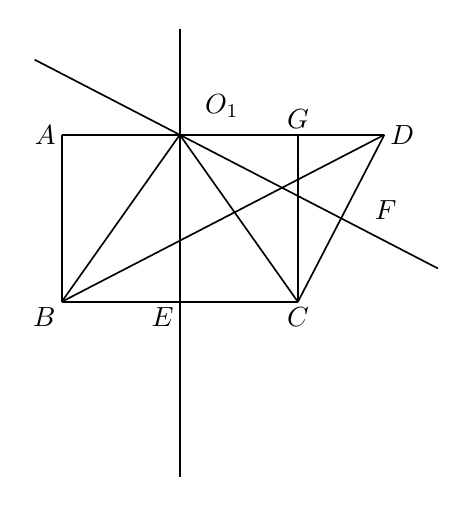
\begin{tikzpicture}[x=1cm,y=1cm,font=\normalsize,
 geometry edge/.style={solid,line width=.6pt},
 geometry mark/.style={solid,line width=.6pt},
 geometry label/.style={font=\normalsize,inner sep=2pt}]
\coordinate (VTop) at (1.500000000,4.350000000);
\coordinate (VBot) at (1.500000000,-1.350000000);
\coordinate (LTop) at (-0.344100000,3.954600000);
\coordinate (LEnd) at (4.778400000,1.302900000);
\coordinate (A) at (0.000000000,3.000000000);
\coordinate (O1) at (1.500000000,3.000000000);
\coordinate (G) at (3.000000000,3.000000000);
\coordinate (D) at (4.098150000,3.000000000);
\coordinate (B) at (0.000000000,0.878700000);
\coordinate (E) at (1.500000000,0.878700000);
\coordinate (C) at (3.000000000,0.878700000);
\coordinate (F) at (3.549000000,1.939350000);
\draw[geometry edge] (A)--(O1)--(G)--(D);
\draw[geometry edge] (B)--(E)--(C);
\draw[geometry edge] (VTop)--(O1)--(E)--(VBot);
\draw[geometry edge] (LTop)--(O1)--(F)--(LEnd);
\draw[geometry edge] (C)--(F)--(D);
\draw[geometry edge] (A)--(B);
\draw[geometry edge] (G)--(C);
\draw[geometry edge] (B)--(O1);
\draw[geometry edge] (O1)--(C);
\draw[geometry edge] (B)--(D);
\node[geometry label,left] at (A) {$A$};
\node[geometry label,above right,xshift=7pt,yshift=4pt] at (O1) {$O_1$};
\node[geometry label,above] at (G) {$G$};
\node[geometry label,right] at (D) {$D$};
\node[geometry label,below left] at (B) {$B$};
\node[geometry label,below left] at (E) {$E$};
\node[geometry label,below] at (C) {$C$};
\node[geometry label,right,xshift=10pt,yshift=3pt] at (F) {$F$};
\end{tikzpicture}
